%!TEX root = main.tex

\subsection{Introduction}

DNA Microarrays measure the level of expression of all genes in a signle experiment. Data measurements $\rightarrow$ Preprocess and sample normalization $\rightarrow$ Gene selection and sample classification $\rightarrow$ Diagnosis, prognosis or prediction of the reponse to a treatment.

The \textbf{gene selection} (supervised learning) to find a subset of genes to predict the response of new samples. There are some \textbf{objectives}:
\begin{itemize}
	\item Insight into the data and the predictive model;
	\item Link between data analysis and medical expert;
	\item Biological validation;
	\item Reduce financial cost.
\end{itemize}

There are some \textbf{difficulties}:
\begin{itemize}
	\item Measurements are noisy;
	\item Gene expression varies due to many factors;
	\item Financial cost;
	\item Small n large p problem.
\end{itemize}

\subsection{Preprocessing}

\subsubsection{Summarization}

Define a single probeset expression level from the various probe intensities. There are popular techniques: MAS 5.0, RMA, GC-RMA. 
\begin{itemize}
	\item background adjustment: optical noise correction, probe affinity adjustment (influenced by the GC content), RMA ignores the MM probes;
	\item sample normalization: quantiles should be stable across samples, after conversion to log intensities for (GC-)RMA;
	\item summarization: median polish.
\end{itemize}

\subsubsection{Feature normalization}

Make sure that each gene (probeset) has roughly the same expression range across all samples and then do a \textbf{Z-score normalization}: Replace $x_{i,j}$ by $\frac{x_{i,j} - \mu_j}{s_j}$. $\mu_j$ is the mean level of expression of probeset j over the training samples and $s_j$ is the tandard deviation.

\subsubsection{Distance between expression values}

\begin{figure}[H]
	\centering
	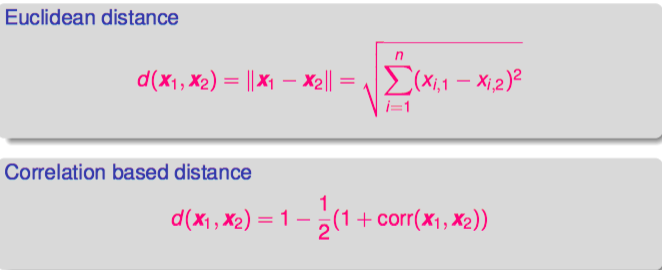
\includegraphics[scale=0.5]{images/51_distance.png}
\end{figure}

\paragraph{Pearson correlation}

\begin{center}
	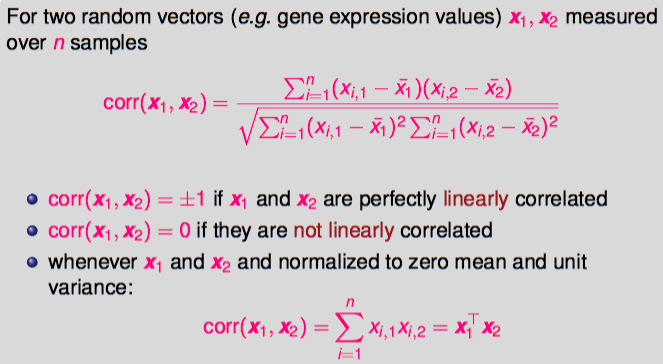
\includegraphics[scale=0.6]{images/52_pearson.png}
\end{center}

\paragraph{Pitfalls with correlation measure}

\begin{center}
	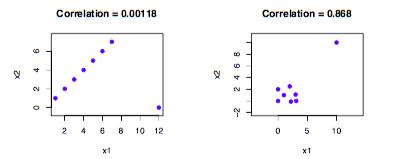
\includegraphics[scale=0.6]{images/53_outliers.png}
	\captionof{figure}{Correlation is sensitive to outliers.}
\end{center}

\begin{center}
	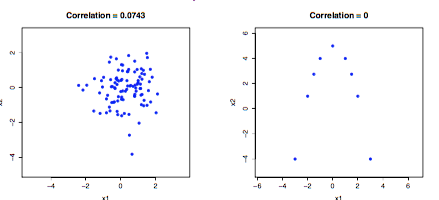
\includegraphics[scale=0.4]{images/54_linear.png}
	\captionof{figure}{Correlation measures \textbf{linear} dependence.}
\end{center}


\paragraph{Spearman's rank correlation}

This correlation is less sensitive to outliers (but still measure linear dependence).
\begin{itemize}
	\item Replace feature value by feature value rank across observations;
	\item Compute pearson correlation between rank vectors.
\end{itemize}

\subsection{Unsupervised learning}

\begin{figure}[H]
	\centering
	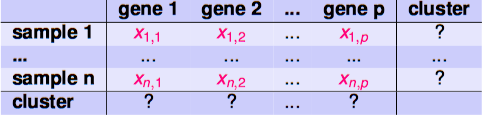
\includegraphics[scale=0.4]{images/50_unsupervised.png}
	\caption{Objective is to find cluster of genes that share similar profile.}
\end{figure}


\begin{figure}[H]
	\centering
	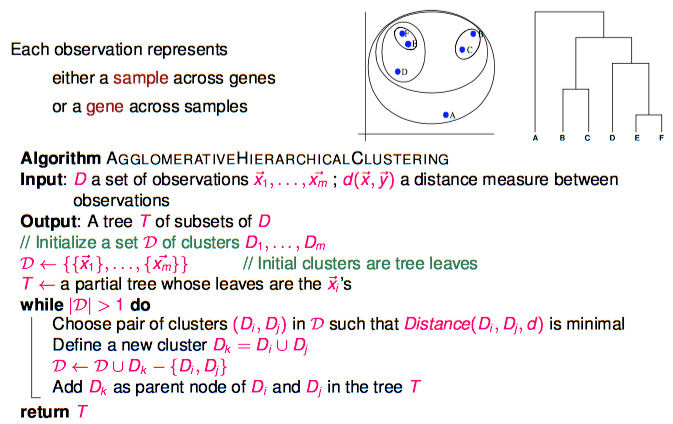
\includegraphics[scale=0.55]{images/55_agglo.png}
	\caption{Agglomerative hierarchical clustering.}
\end{figure}
There are different distance measure between the clusters.

\begin{figure}[htp]
	\centering
	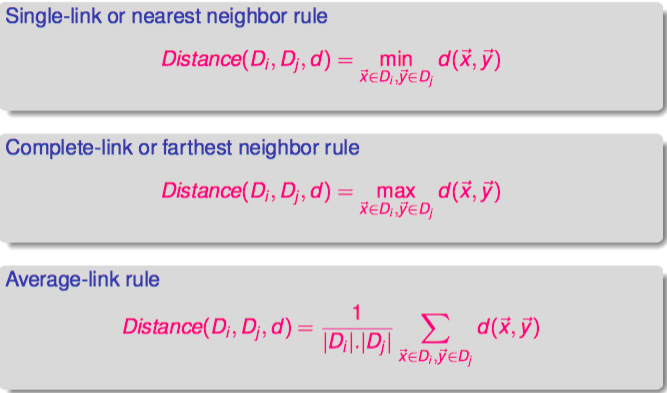
\includegraphics[scale=0.6]{images/56_measure.png}
\end{figure}

\textbf{UPGMA} algorithm is with average-link measure. Used in phylogeny.


\subsection{Supervised learning}

\begin{figure}[htp]
	\centering
	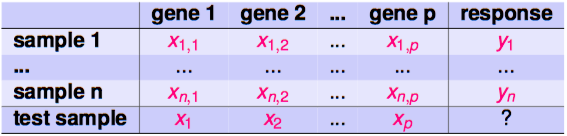
\includegraphics[scale=0.6]{images/49_supervised.png}
	\caption{p input dimensions, n samples, y is binary, natural or real. THe goal is to find the most discriminating genes for the prediction of the class of any new sample.}
\end{figure}

\subsubsection{Filters}

\begin{figure}[H]
	\centering
	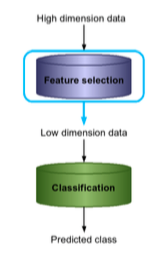
\includegraphics[scale=0.6]{images/57_filters.png}
	\caption{Use only training data and class labels during the features selection step and then train a single classifier taking the selected features as inputs. It is the less computive approach.}
\end{figure}

\paragraph{Non-specific filtering}

Keep only genes with the larger variances (top 25\%) because they are discriminating (do it before normalization to unit variance).


\paragraph{Fold changes}

\begin{center}
	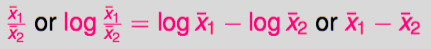
\includegraphics[scale=0.6]{images/60_fold.png}
	\captionof{figure}{Keep genes with larger fold changes between both conditions. Not a good filters because discriminating genes with large difference but small ratio are missed.}
\end{center}

\paragraph{t-Test relevance index}

\begin{center}
	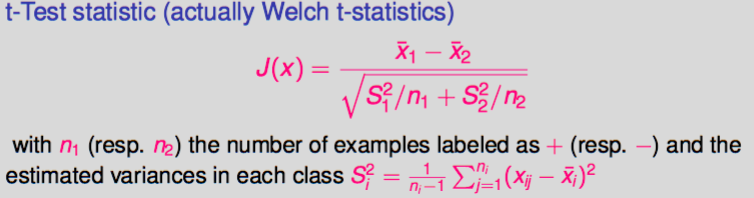
\includegraphics[scale=0.6]{images/61_test.png}
	\captionof{figure}{$J(x)$ is the distance between feature and average feature value in \textbf{each class}. p-values assess the signifiance of the difference between the two class means. A feature is selected if its associated p-value is below a prescribed theshold.}
\end{center}

\subparagraph{Alternatives of the simple t-Test}
\begin{itemize}
	\item Mann-Whitney rank test is an alternative \textbf{non-parametric} test;
	\item ANOVA is a generalization of the t-Test with \textbf{multi-class} (bigger than 2);
	\item Pairwise t-Tests \textbf{between one class and the others};
	\item Kruskal-Wallis is a generalization of M-W (\textbf{non parametric multi class}).
\end{itemize}

\paragraph{Multiple test correction}

It is possible to conclude that the mean expression values among the 2 classes are significantly different for a given gene while they are not. If the test is performed 50000 times and $\alpha = 0,05$, we are expected to wrongly select $50000*0,05=2500$ genes. We need correction.

\subparagraph{Bonferoni correction}

Divide the critical value by the number of tests $n_t$ performed ($\frac{0,05}{50000}$). Tends to select no features.

\subparagraph{False Discovery Rate correction}

\begin{center}
	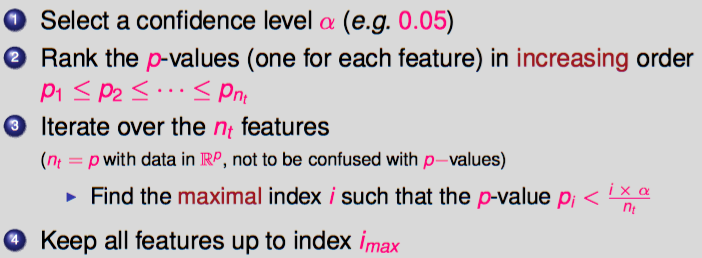
\includegraphics[scale=0.6]{images/62_fdr.png}
	\captionof{figure}{If $p_{n_t} < 0,05$ FDR select all the features. Only the selection threshold is changed.}
\end{center}


\newpage
\paragraph{Feature ranking with mutual information}

\begin{center}
	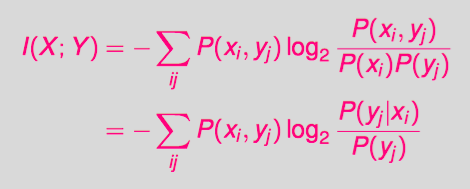
\includegraphics[scale=0.6]{images/63_mutual.png}
	\captionof{figure}{A feature X is more relevant if its mutual information with the class value is higher. If X tend to bring no info to predict Y: $I(X;Y) \rightarrow 0$. $I(X;Y) = 0$ if X and Y independent.}
\end{center}


Those are univariate filters. We can use mutual information to select several variables at a time. 

\paragraph{Maximum relevance minimum redondancy}
\begin{center}
	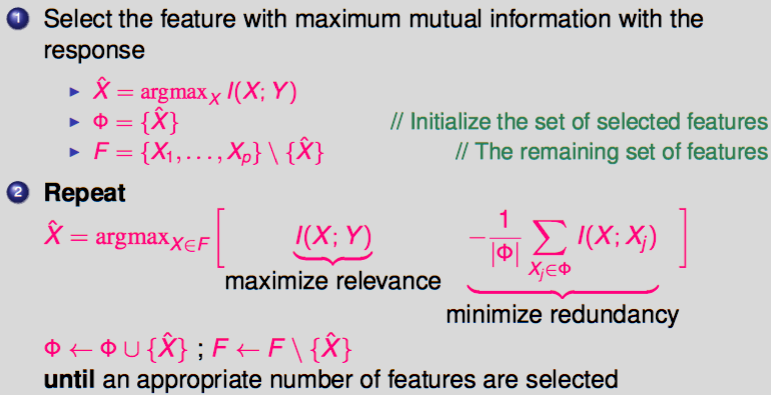
\includegraphics[scale=0.6]{images/64_maxmin.png}
\end{center}

\paragraph{Conclusion}

Filters is the cheapest approach and is useful when we have large number of features. Univariate filters ignore interactions between genes. 

\subsubsection{Wrappers}

\begin{figure}[H]
	\centering
	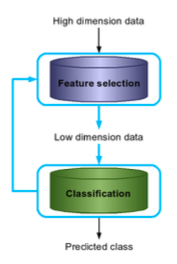
\includegraphics[scale=0.6]{images/58_wrappers.png}
	\caption{Train a classifier on several subsets of all possible features ($O(2^p)$ different subsets). Exhaustive search is impossible, use feature rankin or f/b selection. Select the feature set that optimize the performance of the trained classifier.}
\end{figure}

\begin{figure}[H]
\centering
\begin{minipage}{.5\textwidth}
  \centering
  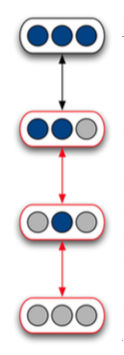
\includegraphics[scale=0.5]{images/65_uni.png}
  \caption{Univariate feature ranking.}
\end{minipage}%
\begin{minipage}{.5\textwidth}
  \centering
  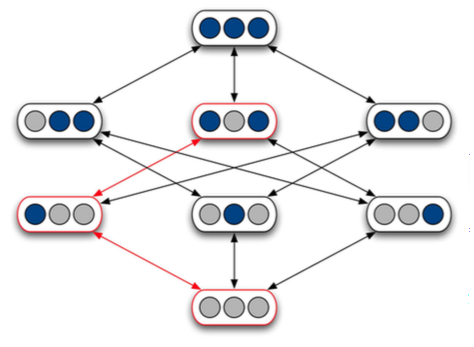
\includegraphics[scale=0.5]{images/66_multi.png}
  \caption{Multivariate Forward (bottum-up, nothing to all) or Backward (top-down, all to nothing) selection.}
\end{minipage}
\end{figure}

The search order matters. If you can afford the computational cost of multivariate selection, you can do an embedded approach.


\subsubsection{Embedded approaches}

\begin{figure}[H]
	\centering
	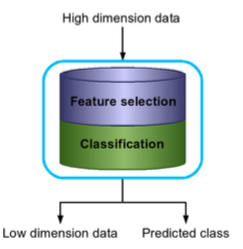
\includegraphics[scale=0.6]{images/59_embedded.png}
	\caption{Feature selection and classifier estimation is the same \textbf{combined optimization process}. We include the classifier optimization in the feature selection process. The most computing expensive.}
\end{figure}

\paragraph{Linear discriminats}

\begin{center}
	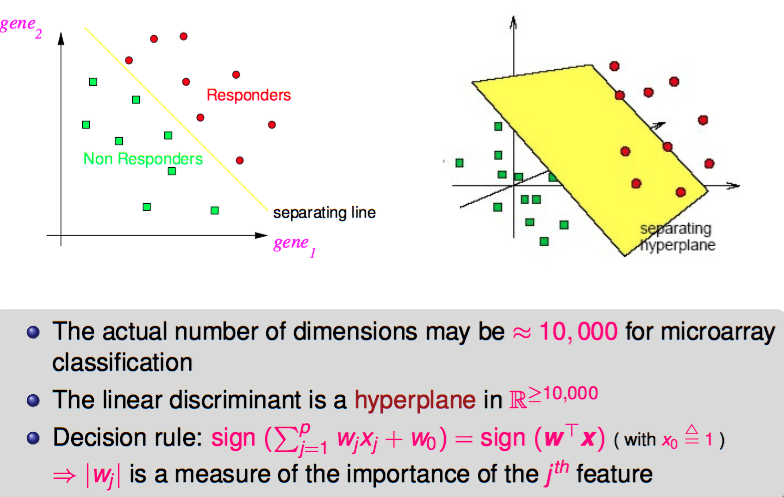
\includegraphics[scale=0.5]{images/67_linear.png}
	\captionof{figure}{The problem is there can be several hyperplane.}
\end{center}
\newpage
\paragraph{Linear Support Vector Machines}

\begin{center}
	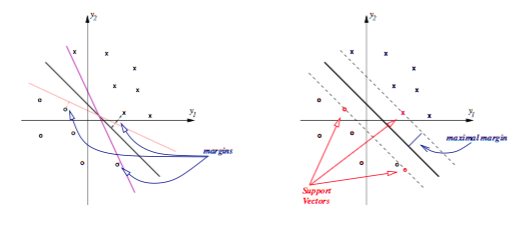
\includegraphics[scale=0.6]{images/68_svm.png}
	\captionof{figure}{SVM. Need to find the maximal margin.}
\end{center}

\paragraph{Recursive feature Elimination}

\begin{center}
	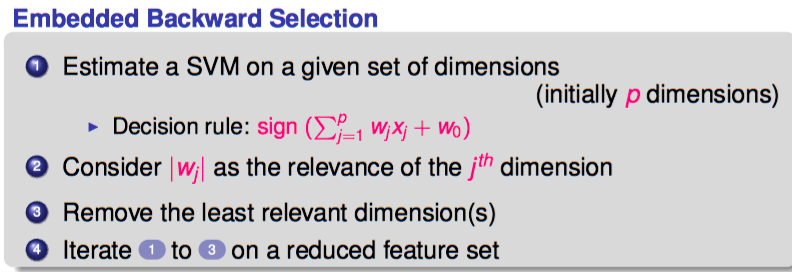
\includegraphics[scale=0.5]{images/69_rec.png}
\end{center}

